\section{Echtzeitvisualisierung und OpenGL}
\subsection{Geschichte}
OpenGL entstand ursprünglich aus dem von Silicon Graphics (SGI) entwickelten IRIS GL. Im sogenannten Fahrenheit-Projekt versuchten Microsoft und SGI ihre 3D-Standards zu vereinheitlichen, das Projekt wurde jedoch wegen finanzieller Schwierigkeiten auf Seiten von SGI abgebrochen.

Der OpenGL-Standard wird vom OpenGL ARB (Architecture Review Board) festgelegt. Das ARB existiert seit 1992 und besteht aus einer Reihe von Firmen. Stimmberechtigte Mitglieder sind die Firmen 3DLabs, Apple, AMD/ATI, Dell, IBM, Intel, Nvidia, SGI und Sun (Stand Nov. 2004). Weiter mitwirkende Firmen sind Evans and Sutherland, Imagination Technologies, Matrox, Quantum3D, S3 Graphics, Spinor GmbH, Tungsten Graphics, und Xi Graphics. Microsoft, eines der Gründungsmitglieder, hat das ARB im März 2003 verlassen.

Neue Funktionen in OpenGL werden meist zuerst als herstellerspezifische Erweiterungen eingeführt und gehen dann den Weg über herstellerübergreifende Erweiterungen und ARB-Erweiterungen zu Kernfunktionalität. Dies erlaubt es, neueste Möglichkeiten der Grafikhardware zu nutzen und dennoch OpenGL abstrakt genug zu halten.

Quelle: https://de.wikipedia.org/wiki/OpenGL
\subsection{GL-Pipeline}
Eine Computergrafik-Pipeline besteht im Wesentlichen aus den folgenden Schritten:
\begin{figure}[H]
    \centering
    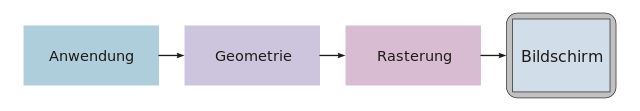
\includegraphics[width=1.0\textwidth]{images/cgpipeline_grob.png}
    \caption{Computergrafik-Pipeline}
    \label{fig:gimbal+lock}
\end{figure}

Eine solche Pipline wird auch von OpenGL implementiert. Es besteht jedoch die Besonderheit, dass die Geometrie und die  Rasterung in Hardware realisiert ist und man durch kleine Programme, sogenannte Shader, auf diese Hardware zugreifen und Manipulationen vornehmen kann beziehungsweise seit OpenGL 2.0 sogar muss.

\subsubsection{Rasterung}
\begin{figure}[H]
    \centering
    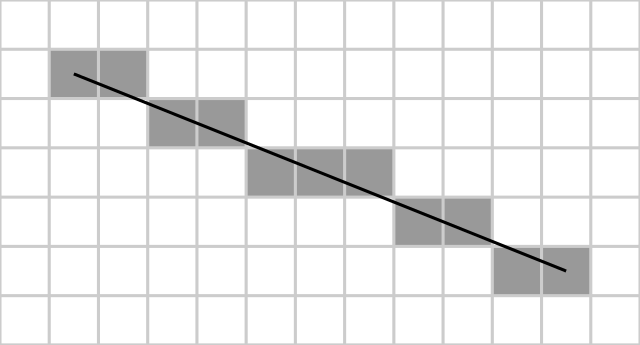
\includegraphics[width=1.0\textwidth]{images/bresenham.png}
    \caption{Bresenham Algorithmus}
    \label{fig:gimbal+lock}
\end{figure}
Als Rasterung bezeichnet man das transformieren kontinuierlicher (geometrischer) Daten auf diskrete Pixel.
Anhand der gegebenen Daten muss also entschieden werden, welche Farbe ein Pixel des Ausgabegerätes erhält.
Eines der elementarsten Algorithmen in diesem Zusammenhang ist der Bresenham Algorithmus, der zur Rasterung von Linien verwendet wird. Alle häufig verwendeten Rasterverfahren für Dreiecke und andere primitiven sind im wesentlichen Abwandlungen und Weiterentwicklungen  des Bresenham Algorithmus.

\subsubsection{Geometrie}
Die Geometrieverarbeitung   besteht aus der Hintereinanderausführung der folgenden affinen/homogenen Abbildungen und Algorithmen:
\begin{figure}[H]
    \centering
    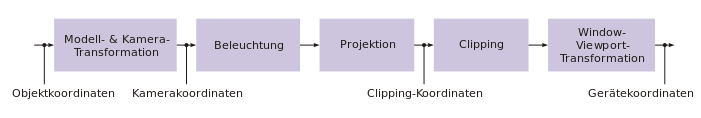
\includegraphics[width=1.0\textwidth]{images/cgpipeline.png}
    \caption{Geometrie-Pipeline}
    \label{fig:gimbal+lock}
\end{figure}

Die Projektion wird durch eine Matrix  ähnlich der Projektionsmatrix $K_{persp_{xy}}$ aus Abschnitt 1.2.1 realisiert.
Es werden jedoch noch ein Translation, eine Rotationen und eine Stauchung dazwischengeschaltet, die ebenfalls als $4 \times 4$ Matrizen realisiert werden können.  Man erreicht damit, dass der Kegelstumpf zwischen der forderen Projektionsebene, auch 'nearplane' genannt,  und der hinteren Ebene, auch 'farplane' genannt, in den $[-1,1] \times [-1,1] \times [-1,1] $ Würfel abgebildet wird.   
\begin{figure}[H]
    \centering
    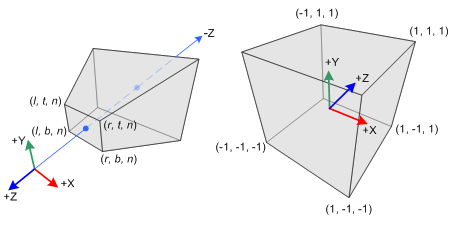
\includegraphics[width=1.0\textwidth]{images/gl_projectionmatrix01.png}
\end{figure}



\begin{Definition}[z-Buffer]
\end{Definition}


\begin{Algorithmus}[z-Buffer-Algorithmus]
\end{Algorithmus}



\begin{figure}[H]
    \centering
    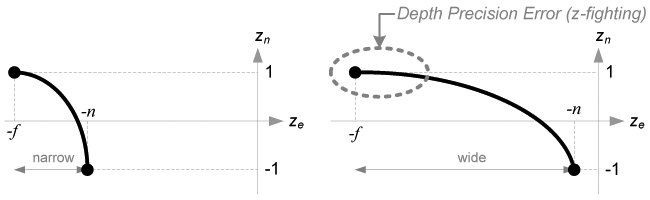
\includegraphics[width=1.0\textwidth]{images/gl_projectionmatrix_zbuffer_1.png}
\end{figure}



\subsection{Lokale Beleuchtungsmodelle}
\subsubsection{Ideale Reflexionen und Lichtbrechungen}
\subsubsection{Lambert  Modell}
\subsubsection{Phong Modell}

\subsection{Texturen und UV-Mapping}
\subsection{Shaderprogrammierung und standard Algorithmen}
\subsubsection{Syntax und Funktionsumfang}
\subsubsection{Flat  shading}
\subsubsection{Phong  shading}
\subsubsection{Bumpmapping}
\subsubsection{Displacementmapping}
\subsubsection{Shadowmap}

\subsection{Labor}
\subsubsection{WebGL}
